% arara: pdflatex: {options: "-draftmode"}
% arara: biber
% arara: pdflatex: {options: "-draftmode"}
% arara: pdflatex: {options: "-file-line-error-style"}
\documentclass[MilwayThesis]{subfiles}
%\setcounter{chapter}{2}
\begin{document}

This dissertation rests on a number of non-standard theoretical assumptions and draws a few non-standard distinctions, which I will defend in this chapter.
My defense of the assumptions, however, will not be an argument that they are true, as the truth of any theoretical statement ultimately depends on the empirical facts.
Rather, my defense will actually be an offense; I will argue that the standard assumption is, in fact, ill-founded.
So, in a sense, I will be rejecting standard assumptions rather than making non-standard ones.
The distinctions I draw, in contrast, will not be defended, but rather explained and clarified.

\section{The $\Theta$-Criterion}
The $\theta$-criterion standardly assumed was first formulated by Chomsky in \textit{Lectures in Government and Binding} (LGB) as \Next.
\ex. Each argument bears one and only one $\theta$-role, and each $\theta$-role is assigned to one and only one argument. \parencite[36]{chomsky1981lectures}

In a footnote, Chomsky justifies this criterion, saying 
\begin{quote}
	The second clause of [the $\theta$-criterion] is well-motivated.
	To say that each $\theta$-role must be filled implies, for example, that a pure transitive verb such as \textit{hit} must have an object, that a verb such as \textit{put} or \textit{keep} (with the sense they have in \textit{put it in the corner}, \textit{keep it in the garage}) must have the associated PP slot filled, etc. 
	The additional requirement that each $\theta$-role must be filled by only one argument will, for example, exclude the possibility that a single trace is associated with several argument antecedents, a possibility ruled out in principle under the Move-$\alpha$ theory. 
	\parencite[139]{chomsky1981lectures}
\end{quote}
I would agree that the second clause of \Last, that each $\theta$-role is assigned to a single argument, is well-motivated by the empirical considerations Chomsky cites, and as such I will not reject that portion of the $\theta$-criterion.
The first clause, however, is motivated mainly by theoretical concerns of LGB, that is, its connection to empirical facts is indirect at best.

The nature of the LGB theory is such that its various hypotheses and principles are connected to each other in a web-like network.
As a result, the first clause of the $\theta$-criterion depends on various other theoretical statements and various other theoretical statements depend on it.
So, rather than attempting an exhaustive enumeration of the links between the $\theta$-criterion and the other theoretical statements of LGB, I will present what I consider to be the best argument in favour or the $\theta$-criterion, and argue that its premises have since been rejected within syntactic theory.

The first premise is the now familiar Y- or T-model of grammar shown in \Next, which LGB theory continues from earlier theories.
According to this model, a syntactic derivation has four levels of representation (D-structure, S-Structure, PF, and LF), and each step in the derivation is performed by the application of a subset of the transformational rules.
S-structures are derived by the applying of Move-$\alpha$ to D-structures, LFs are derived by applying QR (and maybe Move-$\alpha$) to S-structures, and PFs are derived by applying ``stylistic rules'' to S-structures \parencite[18]{chomsky1981lectures}.
\ex. 
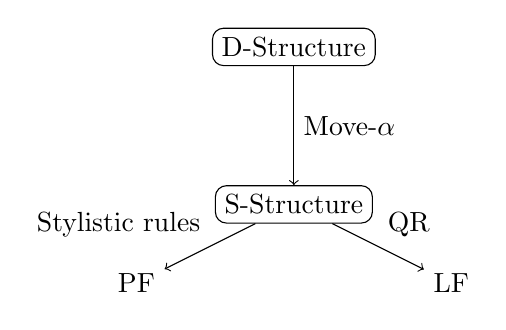
\begin{tikzpicture}[baseline]
	\node[draw,rounded corners] (DS) at (0,0) {D-Structure};
	\node[draw,rounded corners] (SS) at (0,-2) {S-Structure};
	\node (PF) at (-2,-3) {PF};
	\node (LF) at (2,-3) {LF};
	\draw[->] (DS)--(SS) node[midway,right] {Move-$\alpha$};
	\draw[->] (SS)--(PF) node[midway,anchor=south east] {Stylistic rules};
	\draw[->] (SS)--(LF) node[midway,anchor=south west] {QR};
\end{tikzpicture}

The exact natures of the transformations are not important for this discussion.
What is important, is that all syntactic displacement is the result of one of these transformations.

The second premise is the projection principle, which states that lexical properties must be represented at all levels of syntax.
Since $\theta$-roles are lexical properties of (at least) verbs, they must be represented at all levels of syntax.
Consider the verb \textit{hit}, whose lexical entry specifies that it needs a patient argument.
The projection principle requires that at D-Structure and S-Structure \textit{hit} must have assigned a patient $\theta$-role to an argument and therefore, assuming the patient $\theta$-role is assigned to Comp,V, there must be a DP in the complement position of \textit{hit} at both D-Structure and S-Structure.

With these assumptions, it follows that no single argument can receive more than one $\theta$-role.
Suppose there is a derivation in which a single argument X receives two $\theta$-roles $\Theta1$ and $\Theta2$.
According to the projection principle, X must be marked with both $\Theta1$ and $\Theta2$ at D-Structure.
Since each $\theta$-role is associated with a unique structural position, it follows that X must be in two distinct positions at D-Structure.
The only way an argument can be in multiple positions is if it has undergone Move-$\alpha$.
Move-$\alpha$, however, maps D-Structures to S-Structures.
Therefore, an argument cannot be in two positions at D-Structure, and furthermore, cannot be multiply $\theta$-marked at D-Structure.
If an argument cannot be multiply $\theta$-marked at D-Structure, then it cannot be multiply $\theta$-marked at all.

Thus we are able to derive the first clause of the $\theta$-criterion from other principles.
These principles, however, have either been rejected or problematized since their statement in LGB.
Since \textit{The Minimalist Program} \parencite{chomsky1995minimalist}, generative theories have largely dispensed with D-Structure and S-Structure.
Without these levels of representation, the projection principle (as formulated in LGB) is effectively meaningless, and without the projection principle, there is no more basis for the first clause of the $\theta$-criterion.
Therefore, I will not be assuming the first clause of the $\theta$-criterion.

\section{Last Resort}
It almost goes without saying that the goal of the minimalist program is to clean up syntactic theory by explaining unnecessary principles in terms of necessary principles.
In nearly one fell swoop, \textcite{chomsky1995minimalist} eliminates a number of the complications built into LGB theory (S-Structure and D-Structure chief among them).
In \textit{The Minimalist Program} (MP), however, Chomsky was not able to explain two seeming imperfections: displacement and uninterpretable features.\footnote{
	The framework developed in MP also does not explain projection/labelling, but Chomsky does not recognize this as an imperfection until ``Problems of projection'' \parencite{chomsky2013problems}.
	More on this in Chapter \ref{sec:labels}
}
Chomsky formalized displacement as the operation Move, which is more complex than Merge, and proposes that, unlike Merge, which ``comes for free,'' every instance of Move must be triggered by the the need to satisfy an uninterpretable feature.
The simple operation Merge is preferred for economy reasons, while movement, Chomsky argues, is a ``last resort.''
In work subsequent to MP, however, Chomsky proposes that Move is actually a subtype of Merge, called Internal Merge.
Merge and Move are different names for the same operation, there is no reason to think that Move is more computationally complex, and therefore no reason to think that movement is a last resort.

In ``Beyond Explanatory Adequacy'' \parencite[][henceforth, \textit{BEA}]{chomsky2004beyond} Chomsky makes this rejection of Last Resort explicit:
\begin{quote}
	[Narrow Syntax] is based on the free operation Merge.
	[The Strong Minimalist Thesis] entails that Merge of $\alpha$, $\beta$ is unconstrained, therefore either external or internal.
	Under external Merge, $\alpha$ and $\beta$ are separate objects; 
	under internal Merge, one is part of the other, and Merge yields the property of ``displacement,'' which is ubiquitous in language and must be captured in some manner in any theory. 
	It is hard to think of a simpler approach than allowing	internal Merge (a grammatical transformation), an operation that is freely available.
	\parencite[110]{chomsky2004beyond}
\end{quote}
This line of reasoning bears discussion in light of the fact that Last Resort is still standardly assumed by self-described minimalist syntacticians.
In fact, several syntacticians expand Last Resort to External Merge arguing that neither type of Merge ``comes free'' \parencite{pesetsky2006probes,frampton2008crash,wurmbrand2014merge,yokoyama2015features}.
This proposal is understandable from a historical perspective, but ultimately misguided in my opinion.

Perhaps the most attractive aspect of a constrained Merge syntax is the purported gains in computational efficiency.
To illustrate this, \textcite{frampton2008crash} consider the incomplete product of a doomed derivation in \Next
\ex. it to be believed Max to be happy

A free Merge syntax, according to \textcite{frampton2008crash}, the derivation must continue for an indefinite time until a phase head is merged.
At this point the derivation will crash due to a Case Filter violation.
A constrained Merge syntax, however, could be able to halt as soon as the derivation becomes doomed, say, when \textit{it} is merged.
This would save us the indefinite number steps it takes to merge a phase head, and is therefore more efficient.
This I take to be a species of the argument that free Merge systems are inefficient because, in addition to the infinite array of convergent derivations they must generate, they also generate an infinite array of crashing derivations, whereas constrained Merge systems only generate to ``convergent'' derivations.
However, when we investigate the nature of constrained Merge, we can see that the purported gains in efficiency in one part of the system come at the expense of another part of that same system.
Constrained Merge theories, in effect, rob Peter to pay Paul.

At minimum, each version of the syntax will have a Merge operation and a Transfer operation.
So, the free Merge syntax will consist of a unconstrained Merge$_F$ and a constrained Transfer$_F$ as defined in \Next.
\ex.
\a. Merge$_F(\alpha,\beta) = \left\{ \alpha, \beta \right\}$ 
\b. Transfer$_F(\gamma) = \langle\textsc{sem}(\gamma), \textsc{phon}(\gamma)\rangle$ iff Filter($\gamma$) = F\\
(where $\alpha$, $\beta$, and $\gamma$ are syntactic objects.)

A constrained Merge syntax, then, would be consist of a constrained Merge$_C$ and an unconstrained Transfer$_C$.
\ex.
\a. Merge$_C(\alpha,\beta) =$ Merge$_F(\alpha,\beta)$ iff Satisfy($\alpha,\beta$) = T
\b. Transfer$_C(\gamma) = \langle\textsc{sem}(\gamma), \textsc{phon}(\gamma)\rangle$
(where $\alpha$, $\beta$, and $\gamma$ are syntactic objects.)

If we assume that both theories can be made descriptively adequate, then the Satisfy predicate will have the same net effect of the Filter predicate required for the free Merge system.
So, given any pair of syntactic objects $\alpha$ and $\beta$, Satisfy must be able to evaluate if Merge($\alpha,\beta$) is allowed.
And since there are an infinite amount of deriveable syntactic objects, even in a constrained Merge syntax, Satisfy must be able to evaluate an infinity of possible $\beta$'s against each possible $\alpha$.
For any given syntactic object, then, there is an indefinite amount of objects which will merge with that object and an indefinite amount that will not, and the only way to know if Satisfy is true of a pair of objects is to chack.
So, much like free Merge syntax suffers from an infinity of crashes, constrained Merge syntax suffers from an infinity of failed Merge operations.

A constrained Merge theorist, might still object by saying that Satisfy is a local operation, while Filter is a global operation, and local operations are to be preferred if we care about computational complexity.
Again, this is an intuitively attractive argument, but not obviously valid.
Consider the following thought experiment.
Suppose you are a TA charged with grading a quiz by your somewhat maniacal instructor.
Part of the instructor's mania is that they require all quizzes to consist of 40 equally weighted questions and be graded out of 10 points.
What is the most efficient procedure for assigning a grade to each quiz?
Two types of procedure suggest themselves.
The first, which I will call the Local Only procedure, is to assign each correct answer a value of 0.25 points and then add up all of the points.
The second, which I will call the Local/Global procedure, it to assign each correct answer a value of 1 point, add up all of the points, and divide by 4 (perhaps with a calculator).
Since humans are Very Good at counting by increments of 1, and calculators are Very Good at dividing by 4, while neither is Very Good at counting by increments of 0.25, the Local/Global procedure is likely to be more efficient than the Local Only procedure.
The moral of this story: One machine's global procedure is another machine's local procedure.

There is also a methodological rationale for preferring a free Merge framework which is slightly counterintuitive, so I would like to dwell on it for a moment.
My reason for assuming a free Merge framework is that it creates, or rather, lays bare, more problems for us to solve.
So, why is this preferrable?
Shouldn't we prefer the theory with fewer problems?
Inuitively, we should prefer the less problematic theory, but this all depends on how we count a theory's problems.
I would like to argue that, while free Merge theories pose a greater number of problems than constrained Merge theories, the sheer weight of the problems posed by each type of theory is equal to that of the other.
Furthermore, the problems of free Merge can be made into empirical questions more readily than those of constrained Merge.

In order to argue in favour of free Merge, I will present one argument against it and show how that argument actually strengthens my claims in the previous paragraph.
The argument comes from \textcite{frampton2008crash}, and states that a free Merge theory of grammar must posit ``filters'' to rule out the non-converging structures that its syntax generates, and the last thing we want is a flourishing of filters.
I could not agree more with their assessment, but where they see a bug, I see a feature.
So-called ``filters'' are not attempts at explanation, but descriptions of generalizations in need of explanation.

Take, for instance, the remaining clause of the $\theta$-criterion, given in \Next.
\ex. [E]ach $\theta$-role is assigned to one and only one argument. \parencite[36]{chomsky1981lectures}

To propose a $\theta$-filter, then would be to say that those derivations which violate \Last crash at an interface, presumably the CI interface.
For a theorist, this filter is actually a question or series of questions: Why is it that only those derived structures which satisfy \Last are valid CI objects?
That question may not be empirical, but it invites hypotheses which may lead to empirical questions which we don't currently know how to ask.
Very likely, due to the interface-nature of the questions, their answers will not be narrowly linguistic.

Now, consider the situation constrained Merge puts the theorist in.
For \textcite{frampton2008crash}, the $\theta$-criterion is expressed by ``selectional features'' on heads which must be satisfied immediately.
This leads to a number of questions: What is the nature of these selectional features?
How are they related to, say, $\varphi$-features?
Do they exist independently of the narrow syntax?
Why do they need to be satisfied first?
And so on.
I, for one, don't have the slightest clue how to proceed in answering or even sharpening these questions, and there don't seem to be any clues in the offing from constrained Merge theorists.

\section{Terminological notes}
The subject matter of this thesis is often called the ``syntax-semantics interface,'' a term which I have discovered is ambiguous, probably due to the fact that it is constructed from three ambiguous terms.

The term \textit{syntax} has (at least) three senses which seem to be used in generative grammar circles.
The first sense, which I will call the sociological sense, is that \textit{syntax} is what syntacticians do.
For instance, $\theta$-theory belongs to the domain of syntax under this sense, because syntacticians care about it, while semanticists tend not to.
However, $\theta$-theory deals at least partially with meaning, so it, at least, intersects with semantics.
This sense would be useful if this dissertation were an intellectual history of generative syntax, but since this is a work of syntactic theory, I will not use this sense.

The second sense, which I will call the broad sense, is that \textit{syntax} is the study (or description) of the form and arrangement of symbolic representations.
Under this sense, the study of syntax would be a part of the study of logic, programming languages, arithmetic, etc.
Furthermore,\textcite[174]{chomsky2000new}, discussing this sense, argues that most of what we call \textit{semantics} and \textit{phonology} would be classified as syntax under this sense.\footnote{Based on my discussion of this sense with phonologists and semanticists, this may be the most controversial claim Chomsky has ever made.}
This sense will prove useful in this dissertation, so I will retain it.

The third sense, which I will call the narrow sense, is that \textit{syntax} is a mental module characterized by a computational procedure that generates an unbounded array of structured form\footnote{I use the term \textit{form} here to refer to all possible expressive modalities of language}-meaning pairs.
This, I believe, is what generative syntacticians mean when they use the term \textit{syntax}.
The ``syntax module'' is one of the objects of study of this thesis, so I will retain this sense.

Since both the broad and narrow senses are useful to me, I will need to make a distinction for the sake of clarity.
I will use the term ``Narrow Syntax'' (or NS) to refer to the narrow sense, that is, the hypothesized mental module, and ``syntax'' (and derived terms) to indicate the broad sense.

Similar remarks apply to the term \textit{semantics}, which has at least three senses.
The first sense, as in the case of \textit{syntax}, is the sociological sense: semantics is what semanticists do.
I will not be using this sense for the same reasons as I cited above for the sociological sense of \textit{syntax}.

The broad sense of \textit{semantics} is that of the study of the relation of a symbolic system to some other system.
So, to various degrees, we can talk about the semantics of a logical system, a programming language, a natural language, etc.
I will use this sense only informally, when discussing notions of truth and reference associated with an instance or class of natural language expression.

The narrow sense of \textit{semantics} is that of the mental module (or system of modules) associated with computing the meaning of a linguistic expression.
Chomsky often refers to this mental entity as the Conceptual-Intentional (CI) system, and stresses that we know very little about it.
Insofar as this thesis makes claims or hypotheses about \textit{semantics}, it makes claims or hypotheses about the CI system.

The final ambiguous term I will discuss is \textit{interface}.
In recent years it has become common within generative linguistics to write papers, hold workshops, and compile books on \textit{the syntax-semantics interface}, but as I mentioned above, the term is ambiguous.
It largely seems to be ambiguous between a \textit{sociological} sense and a \textit{narrow} sense, with the sociological sense dominating discussion.

When used in the sociological sense, the syntax-semantics interface refers to a body of literature that mixes the formalisms and methods used by syntacticians with those used by semanticists.
That is, this type of work makes use of tree diagrams and expressions of typed lambda calculus.
In this sense, the interface is not an object of study per se, but a sub-discipline.

In the narrow sense, the syntax-semantics interface refers to the interface between the Narrow Syntax and the CI system.
This results in very different sorts of analyses compared to the standard analyses, analyses that posit computational procedures rather than merely representing expressions in two ways.
In many ways, however, the term \textit{interface} in its narrow sense is a misnomer, as there are likely no mental objects that we might call interfaces.
As best we can tell, the mind consists of a set of modules and a non-modular central system \parencite{fodor1983modularity,fodor2001mind}.
An interface, then, emerges wherever two modules interact with each other, or perhaps where a module interacts with the central system.
Restricting ourselves to the modules, we can see why positing interfaces as mental objects won't do.
Suppose we have two modules, M1 and M2, which seem to interact with each other.
Being modules, each will consist in a set of computational operations (P1 and P2) defined over a class of syntactically structured (in the broad sense) objects (L1 and L2).
Suppose we posit an interface I1, which consists in an operation P3 that converts objects of L1 into objects of L2.
What is I1, then, but a module that has interfaces with M1 and M2?
If I1 is a module, are its interfaces with M1 and M2 also modules?
If so, then we seem to be stuck with an infite regress.
If not, then interfaces are a special kind of module, but this would raise further questions with respect to their evolutionary origins.

If there are no mental objects that we might call interfaces, then how are we to study them?
The answer to this question is that, to study an interface, we must study the modules associated with that interface with the added assumption that such an interface exists.
So, studying the syntax-semantics interface involves studying the Narrow Syntax and the CI module with the assumption that there is an interface between them.
We will get a glimpse of how such a study would work in chapter \ref{sec:labels}.

\section{Summary}
In this chapter, I have made explicit two of my assumptions which would be considered non-standard among contemporary generative syntacticians.
In particular, I am not assuming the $\theta$-criterion as it is commonly stated, and I am assuming a free Merge syntax.
I have also clarified some terminology that many take for granted, specifically I clarified my use of the term \textit{syntax-semantics interface} and its constituent terms.
Now that the reader has a sense of my theoretical idiosyncrasies, we can move on to more specific concerns in the following chapters.
\end{document}
